\documentclass[]{elsarticle} %review=doublespace preprint=single 5p=2 column
%%% Begin My package additions %%%%%%%%%%%%%%%%%%%
\usepackage[hyphens]{url}



\usepackage{lineno} % add
\providecommand{\tightlist}{%
  \setlength{\itemsep}{0pt}\setlength{\parskip}{0pt}}

\usepackage{graphicx}
\usepackage{booktabs} % book-quality tables
%%%%%%%%%%%%%%%% end my additions to header

\usepackage[T1]{fontenc}
\usepackage{lmodern}
\usepackage{amssymb,amsmath}
\usepackage{ifxetex,ifluatex}
\usepackage{fixltx2e} % provides \textsubscript
% use upquote if available, for straight quotes in verbatim environments
\IfFileExists{upquote.sty}{\usepackage{upquote}}{}
\ifnum 0\ifxetex 1\fi\ifluatex 1\fi=0 % if pdftex
  \usepackage[utf8]{inputenc}
\else % if luatex or xelatex
  \usepackage{fontspec}
  \ifxetex
    \usepackage{xltxtra,xunicode}
  \fi
  \defaultfontfeatures{Mapping=tex-text,Scale=MatchLowercase}
  \newcommand{\euro}{€}
\fi
% use microtype if available
\IfFileExists{microtype.sty}{\usepackage{microtype}}{}
\bibliographystyle{elsarticle-harv}
\usepackage{longtable}
\ifxetex
  \usepackage[setpagesize=false, % page size defined by xetex
              unicode=false, % unicode breaks when used with xetex
              xetex]{hyperref}
\else
  \usepackage[unicode=true]{hyperref}
\fi
\hypersetup{breaklinks=true,
            bookmarks=true,
            pdfauthor={},
            pdftitle={Which Stems Will Beaver Harvest? A Final Project for FOR 796.},
            colorlinks=false,
            urlcolor=blue,
            linkcolor=magenta,
            pdfborder={0 0 0}}
\urlstyle{same}  % don't use monospace font for urls

\setcounter{secnumdepth}{5}
% Pandoc toggle for numbering sections (defaults to be off)

% Pandoc citation processing
\newlength{\cslhangindent}
\setlength{\cslhangindent}{1.5em}
\newlength{\csllabelwidth}
\setlength{\csllabelwidth}{3em}
% for Pandoc 2.8 to 2.10.1
\newenvironment{cslreferences}%
  {}%
  {\par}
% For Pandoc 2.11+
\newenvironment{CSLReferences}[2] % #1 hanging-ident, #2 entry spacing
 {% don't indent paragraphs
  \setlength{\parindent}{0pt}
  % turn on hanging indent if param 1 is 1
  \ifodd #1 \everypar{\setlength{\hangindent}{\cslhangindent}}\ignorespaces\fi
  % set entry spacing
  \ifnum #2 > 0
  \setlength{\parskip}{#2\baselineskip}
  \fi
 }%
 {}
\usepackage{calc}
\newcommand{\CSLBlock}[1]{#1\hfill\break}
\newcommand{\CSLLeftMargin}[1]{\parbox[t]{\csllabelwidth}{#1}}
\newcommand{\CSLRightInline}[1]{\parbox[t]{\linewidth - \csllabelwidth}{#1}\break}
\newcommand{\CSLIndent}[1]{\hspace{\cslhangindent}#1}

% Pandoc header
\usepackage{booktabs}
\usepackage{longtable}
\usepackage{array}
\usepackage{multirow}
\usepackage{wrapfig}
\usepackage{float}
\usepackage{colortbl}
\usepackage{pdflscape}
\usepackage{tabu}
\usepackage{threeparttable}
\usepackage{threeparttablex}
\usepackage[normalem]{ulem}
\usepackage{makecell}
\usepackage{xcolor}



\begin{document}
\begin{frontmatter}

  \title{Which Stems Will Beaver Harvest? A Final Project for FOR 796.}
      
  \begin{abstract}
  North American beaver (Castor canadensis) populations are rebounding following
  regional extirpation throughout North America, leading to increased concern
  about the impacts beaver may have on communities as their populations increase.
  As central place foragers, beaver restructure riparian forest communities
  through the selective cutting of preferred woody species and size classes.
  Being able to predict which stems are likely to be harvested and which areas
  have a high abundance of desirable forage would allow land managers and
  ecologists to identify likely areas for beaver recolonization, enabling
  proactive management to encourage or deter population reestablishment
  as appropriate.\\
  To this end, we fit three models -- a logistic regression, random forest
  classifier, and a stochastic gradient boosting machine as implemented in
  LightGBM -- to try and predict which stems would be harvested by beaver using
  data collected from riparian zones within New York State's Adirondack Park.
  Using tree species, stem size class, waterbody type (stream or lake), and
  distance from waterbodies as predictors, we found that all three methods
  produce highly accurate predictions, with logistic regression producing the
  classifier with the highest AUC and overall accuracy. These models can be used
  to inform forest management practices as beaver populations, and the impacts
  associated with them, continue to proliferate throughout northeastern North
  America.
  \end{abstract}
  
 \end{frontmatter}

\hypertarget{introduction}{%
\section{Introduction}\label{introduction}}

The North American beaver (\emph{Castor canadensis}) is an ecosystem engineer,
inducing landscape-level changes in hydrology and forest structure through a
combination of damming and foraging behaviors. By selectively harvesting stems,
beaver are capable of fundamentally altering forest size structure and species
composition. While this selection process has long been thought to primarily
reflect preferences for individual species (Raffel et al. 2009), recent work has
suggested that beaver select stems principally based upon stem size and distance
from a waterbody, which in turn are highly predictive of stem species within a
given ecosystem (Mahoney and Stella 2020). No matter the mechanism of selection, beaver are
known to preferentially colonize areas with more desirable food stock, and are
more likely to abandon areas once the supply of desirable woody forage has been
exhausted. As a result, being able to predict which stems are more likely to be
harvested by beaver may allow us to predict which areas are more desirable for
beaver recolonization, enabling land managers and ecologists to proactively
manage landscapes to promote or deter beaver activity.

To this end, we set out to produce models to predict which stems would be
harvested by beaver. Using a dataset collected from 19 waterbodies within
New York State's Adirondack State Park (Mahoney and Stella 2020), we used logistic
regression, random forest, and stochastic gradient boosting machine (GBM) models
to attempt to classify stems as either harvested by beaver or non-harvested.
Accurate classifiers would be useful in order to predict areas which are likely
to host future beaver populations as the species continues to recover from
regional extirpation, and would be highly useful for landscape management in
the years to come.

\hypertarget{methods}{%
\section{Methods}\label{methods}}

\hypertarget{field-data}{%
\subsection{Field Data}\label{field-data}}

Data was collected between May and August 2018 as part of a study of beaver
foraging habits within New York's Adirondack State Park (Mahoney and Stella 2020). The
data is structured as a data frame with 1543 observations of
5 variables.

The following variables were recorded:

\begin{itemize}
\tightlist
\item
  Distance of the plot centroid from the riparian area.
\item
  USDA Forest Service common name for each tree. If the tree
  or stump could not be identified down to species level, phylum was recorded
  instead.
\item
  Tree diameter at breast height in centimeters.
\item
  Whether the tree was located within the riparian area of a lake or a stream.
\item
  Whether or not the tree was harvested.
  0 live stems and
  0 harvested stems were recorded. Due to the relatively
  similar number of live and harvested stems, this dataset was considered to
  have balanced classes and no resampling or weighting of classes was performed.
\end{itemize}

For more information, see Mahoney and Stella (2020).

\hypertarget{models}{%
\subsection{Models}\label{models}}

All models were fit to a random 80\% subsample of the original data set, with the
remaining 20\% reserved as a hold-out set.

Three classification models were evaluated.
The first of these was a simple
logistic regression model which incorporated all predictors without interaction
effects to predict probability of harvest.

The second model evaluated was a random forest, fit using the ranger R package
(Wright and Ziegler 2017). Model tuning was done using a random grid search, evaluating 1,000
randomly selected combinations of hyperparameters. The set of hyperparameters
which maximized AUC were selected, with the final model being fit using 12,500
trees, 2 variables per split (``mtry''), and minimum of 15 observations per leaf
node, with trees fit to data sampled with replacement from the training data
set, with each resample 74\% the size of the original training data.

The third and final model evaluated was a stochastic gradient boosting machine,
fit using the lightgbm package (Ke et al. 2021). Model tuning was done using
iterative grid searches, evaluating progressively narrower ranges of multiple
hyperparameters with each iteration. The set of hyperparameters
which maximized AUC were selected, with the final model being fit using 3,000
trees allowed to grow to arbitrary depths, with a learning rate of 0.1 and a
minimum of 13 observations per leaf node. Each tree was fit to a bootstrap
sample that was 90\% the size of the original training data, with a new sample
taken every 5 trees, and each tree was fit using a randomly selected 30\% of
all features.

All models were fit using methods to predict class probabilities, in order to
produce ROC curves and AUC estimates. Classifications were then made using the
thresholds which optimized both sensitivity and specificity, as identified using
the training data. Models were assessed using their overall accuracy,
sensitivity, specificity, and AUC, calculated against the 20\% holdout set.
ROC curves and AUC were calculated using the pROC package (Robin et al. 2011). Data
wrangling used the dplyr, tidyr, and recipes packages (Wickham et al. 2021; Wickham 2021; Kuhn and Wickham 2021).
Manuscript preparation used the ggplot2 and kableExtra packages (Wickham 2016; Zhu 2021).
All
analyses used the R statistical modeling software (R Core Team 2021).

\hypertarget{results}{%
\section{Results}\label{results}}

Model accuracies are reported in Table \ref{tab:accuracy}.
Logistic regression produced the model with the highest AUC, overall accuracy,
and sensitivity, while the stochastic GBM fit through LightGBM provided the
highest specificity. The random forest model performed the worst on all accuracy
measured. ROC curves for each model are presented in Figure \ref{fig:roc}.

\begin{table}

\caption{\label{tab:accuracy}Selected loss functions for logistic, random forest, and stochastic gradient boosting machine models predicting probability of a stem being harvested by beaver.}
\centering
\begin{tabular}[t]{llll}
\toprule
\multicolumn{1}{c}{} & \multicolumn{1}{c}{Logistic Regression} & \multicolumn{1}{c}{Random Forest} & \multicolumn{1}{c}{LightGBM}\\
\midrule
Accuracy & 0.819 & 0.786 & 0.803\\
\addlinespace
Sensitivity & 0.827 & 0.788 & 0.779\\
\addlinespace
Specificity & 0.802 & 0.782 & 0.851\\
\addlinespace
AUC & 0.905 & 0.820 & 0.898\\
\bottomrule
\end{tabular}
\end{table}

\begin{figure}
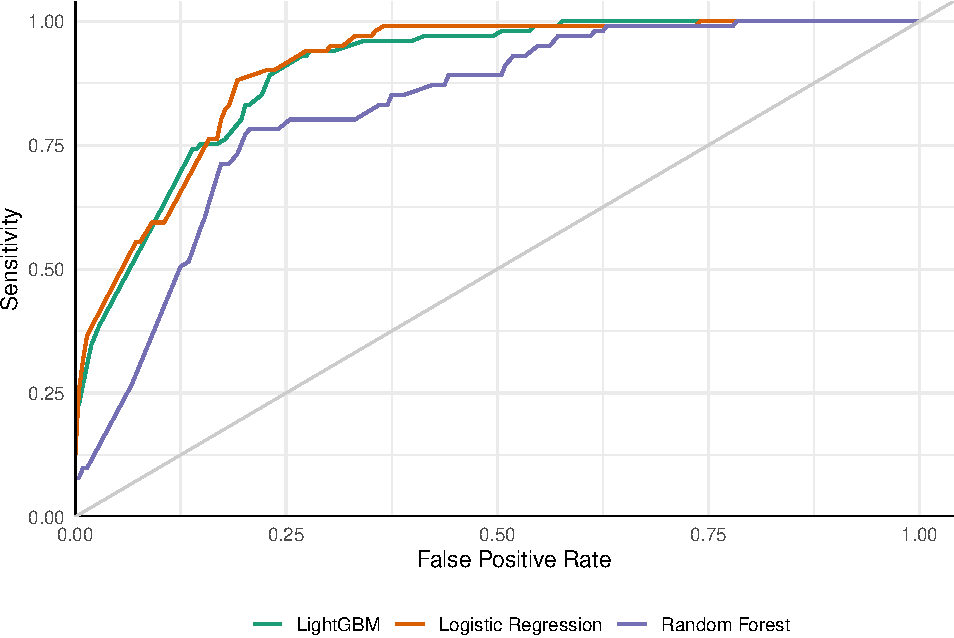
\includegraphics[width=1\linewidth]{project_example_files/figure-latex/roc-1} \caption{ROC curves for three models of probability of stem harvest by beaver.}\label{fig:roc}
\end{figure}

\hypertarget{discussion}{%
\section{Discussion}\label{discussion}}

Given the relatively small data models were built with, it's unsurprising that
the simple baseline model of logistic regression out-performed more complex
alternatives such as random forests and LightGBM. It is likely that with more
predictors or more noisy data the machine learning methods would become more
competitive; however, for this application, the best approach would likely be to
not use machine learning at all.

We could potentially see better results by ensembling these models together,
basing weights either upon a validation set or from a cross validation
procedure. Given that there are 51 observations (approximately 16.5\% of the test
set) where the models produce different predictions, this additional step might
result in significant improvements in predictive accuracy overall.

These models demonstrate the ability to predict the probability of beaver
harvest for riparian trees based on stem size class, species, and distance from
beaver-inhabited waterbodies. This information can be used to inform forest
management practices such as the management of riparian buffers and wildlife
habitat enhancement as beaver populations, and the impacts associated with them,
continue to proliferate throughout northeastern North America.

\newpage{}

\hypertarget{references}{%
\section*{References}\label{references}}
\addcontentsline{toc}{section}{References}

\hypertarget{refs}{}
\begin{CSLReferences}{1}{0}
\leavevmode\hypertarget{ref-lightgbm}{}%
Ke, Guolin, Damien Soukhavong, James Lamb, Qi Meng, Thomas Finley, Taifeng Wang, Wei Chen, Weidong Ma, Qiwei Ye, and Tie-Yan Liu. 2021. \emph{Lightgbm: Light Gradient Boosting Machine}. \url{https://CRAN.R-project.org/package=lightgbm}.

\leavevmode\hypertarget{ref-recipes}{}%
Kuhn, Max, and Hadley Wickham. 2021. \emph{Recipes: Preprocessing Tools to Create Design Matrices}. \url{https://CRAN.R-project.org/package=recipes}.

\leavevmode\hypertarget{ref-Mahoney2020}{}%
Mahoney, Michael J., and John C. Stella. 2020. {``Stem Size Selectivity Is Stronger Than Species Preferences for Beaver, a Central Place Forager.''} \emph{Forest Ecology and Management} 475: 118331. \url{https://doi.org/10.1016/j.foreco.2020.118331}.

\leavevmode\hypertarget{ref-R}{}%
R Core Team. 2021. \emph{R: A Language and Environment for Statistical Computing}. Vienna, Austria: R Foundation for Statistical Computing. \url{https://www.R-project.org/}.

\leavevmode\hypertarget{ref-Raffel2009}{}%
Raffel, Thomas R., Nicole Smith, Catherine Cortright, and A John Gatz. 2009. {``{Central Place Foraging by Beavers (Castor canadensis) in a Complex Lake Habitat}.''} \emph{The American Midland Naturalist} 162 (1): 62--73. \url{https://doi.org/10.1674/0003-0031-162.1.62}.

\leavevmode\hypertarget{ref-pROC}{}%
Robin, Xavier, Natacha Turck, Alexandre Hainard, Natalia Tiberti, Frédérique Lisacek, Jean-Charles Sanchez, and Markus Müller. 2011. {``pROC: An Open-Source Package for r and s+ to Analyze and Compare ROC Curves.''} \emph{BMC Bioinformatics} 12: 77.

\leavevmode\hypertarget{ref-ggplot2}{}%
Wickham, Hadley. 2016. \emph{Ggplot2: Elegant Graphics for Data Analysis}. Springer-Verlag New York. \url{https://ggplot2.tidyverse.org}.

\leavevmode\hypertarget{ref-tidyr}{}%
---------. 2021. \emph{Tidyr: Tidy Messy Data}. \url{https://CRAN.R-project.org/package=tidyr}.

\leavevmode\hypertarget{ref-dplyr}{}%
Wickham, Hadley, Romain François, Lionel Henry, and Kirill Müller. 2021. \emph{Dplyr: A Grammar of Data Manipulation}. \url{https://CRAN.R-project.org/package=dplyr}.

\leavevmode\hypertarget{ref-ranger}{}%
Wright, Marvin N., and Andreas Ziegler. 2017. {``{ranger}: A Fast Implementation of Random Forests for High Dimensional Data in {C++} and {R}.''} \emph{Journal of Statistical Software} 77 (1): 1--17. \url{https://doi.org/10.18637/jss.v077.i01}.

\leavevmode\hypertarget{ref-kableExtra}{}%
Zhu, Hao. 2021. \emph{kableExtra: Construct Complex Table with 'Kable' and Pipe Syntax}. \url{https://CRAN.R-project.org/package=kableExtra}.

\end{CSLReferences}


\end{document}
